
\documentclass[notes,serif]{beamer}
\usepackage{graphicx}
\usepackage{url}
\usepackage{clrscode}
\usepackage{amssymb,amsmath}

% You should run 'pdflatex' TWICE, because of TOC issues.

\mode<presentation>
{
  % A tip: pick a theme you like first, and THEN modify the color theme, and then add math content.
  % Warsaw is the theme selected by default in Beamer's installation sample files.

  %%%%%%%%%%%%%%%%%%%%%%%%%%%% THEME
  %\usetheme{AnnArbor}
  %\usetheme{Antibes}
  %\usetheme{Bergen}
  %\usetheme{Berkeley}
  %\usetheme{Berlin}
  %\usetheme{Boadilla}
  %\usetheme{boxes}
  %\usetheme{CambridgeUS}
  %\usetheme{Copenhagen}
  %\usetheme{Darmstadt}
  %\usetheme{default}
  %\usetheme{Dresden}
  %\usetheme{Frankfurt}
  %\usetheme{Goettingen}
  %\usetheme{Hannover}
  %\usetheme{Ilmenau}
  %\usetheme{JuanLesPins}
  %\usetheme{Luebeck}
  %\usetheme{Madrid}
  %\usetheme{Malmoe}
  %\usetheme{Marburg}
  %\usetheme{Montpellier}
  %\usetheme{PaloAlto}
  %\usetheme{Pittsburgh}
  %\usetheme{Rochester}
  %\usetheme{Singapore}
  %\usetheme{Szeged}
  \usetheme{Warsaw}

  %%%%%%%%%%%%%%%%%%%%%%%%%%%% COLOR THEME
  %\usecolortheme{albatross}
  %\usecolortheme{beetle}
  %\usecolortheme{crane}
  \usecolortheme{default}
  %\usecolortheme{dolphin}
  %\usecolortheme{dove}
  %\usecolortheme{fly}
  %\usecolortheme{lily}
  %\usecolortheme{orchid}
  %\usecolortheme{rose}
  %\usecolortheme{seagull}
  %\usecolortheme{seahorse}
  %\usecolortheme{sidebartab}
  %\usecolortheme{structure}
  %\usecolortheme{whale}

  %%%%%%%%%%%%%%%%%%%%%%%%%%%% OUTER THEME
  %\useoutertheme{default}
  %\useoutertheme{infolines}
  %\useoutertheme{miniframes}
  %\useoutertheme{shadow}
  %\useoutertheme{sidebar}
  %\useoutertheme{smoothbars}
  %\useoutertheme{smoothtree}
  %\useoutertheme{split}
  %\useoutertheme{tree}

  %%%%%%%%%%%%%%%%%%%%%%%%%%%% INNER THEME
  %\useinnertheme{circles}
  %\useinnertheme{default}
  %\useinnertheme{inmargin}
  %\useinnertheme{rectangles}
  %\useinnertheme{rounded}

  %%%%%%%%%%%%%%%%%%%%%%%%%%%%%%%%%%%

%  \setbeamercovered{transparent} % or whatever (possibly just delete it)
  \setbeamercovered{invisible} % or whatever (possibly just delete it)
  % To change behavior of \uncover from graying out to totally invisible, can change \setbeamercovered to invisible instead of transparent. apparently there are also 'dynamic' modes that make the amount of graying depend on how long it'll take until the thing is uncovered.

}


% Get rid of nav bar
\beamertemplatenavigationsymbolsempty

% Use short top
%\usepackage[headheight=12pt,footheight=12pt]{beamerthemeboxes}
%\addheadboxtemplate{\color{black}}{
%\hskip0.3cm
%\color{white}
%\insertshortauthor \ \ \ \
%\insertframenumber \ \ \ \ \ \ \
%\insertsection \ \ \ \ \ \ \ \ \ \ \ \ \ \ \ \ \  \insertsubsection
%\hskip0.3cm}
%\addheadboxtemplate{\color{black}}{
%\color{white}
%\ \ \ \
%\insertsection
%}
%\addheadboxtemplate{\color{black}}{
%\color{white}
%\ \ \ \
%\insertsubsection
%}

% Insert frame number at bottom of the page.
\usefoottemplate{\hfil\tiny{\color{black!90}\insertframenumber}}

\usepackage[english]{babel}
\usepackage[latin1]{inputenc}

\usepackage{times}
\usepackage[T1]{fontenc}

\title{Network Programming}
\subtitle{Lecture 3---Elementary Sockets II: I/O Multiplexing}

\author{Lei Wang\\ lei.wang@dlut.edu.cn}

\institute{Dalian University of Technology}

%\date{Date}
\date{Dec 3, 2008}

\subject{Talks}

\def\defn#1{{\color{red} #1}}

\begin{document}

\begin{frame}
  \titlepage
\end{frame}

\begin{frame}
  \frametitle{Part 2. Elementary Sockets II: I/O Multiplexing}
  \tableofcontents
\end{frame}

\section{I/O Multiplexing: {\tt select} and {\tt poll} function}
\subsection{Introduction}

\begin{frame}
\frametitle{Introduction}

I/O multiplexing is typically used in the following scenarios:
\begin{itemize}
  \item When a client is handling multiple descriptors (normally interactive input and a network socket).
  \item It is possible, but rare, for a client to handle multiple sockets at the same time.
  \item If a TCP server handles both a listening socket and its connected sockets.
  \item If a server handles both TCP and UDP.
  \item If a server handles multiple services and perhaps multiple protocols (e.g., the inetd daemon).
\end{itemize}
Note: I/O multiplexing is not limited to network programming.
\end{frame}

\subsection{I/O Models}
\begin{frame}
\frametitle{I/O Models}
\begin{itemize}
  \item blocking I/O
  \item nonblocking I/O
  \item I/O multiplexing (\texttt{select} and \texttt{poll})
  \item signal driven I/O (\texttt{SIGIO})
  \item asynchronous I/O (the POSIX \texttt{aio\_}functions)
\end{itemize}
\end{frame}

\begin{frame}
\frametitle{Blocking I/O Model}
  \begin{center}
  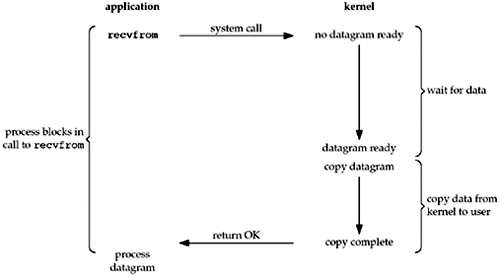
\includegraphics[width=.9\textwidth]{figs/06fig01.png}
  \end{center}
\end{frame}

\begin{frame}
\frametitle{Nonblocking I/O Model}
  \begin{center}
  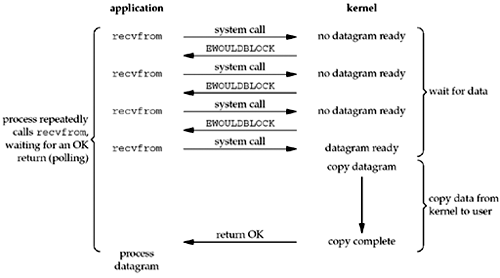
\includegraphics[width=.9\textwidth]{figs/06fig02.png}
  \end{center}
\end{frame}

\begin{frame}
\frametitle{I/O Multiplexing Model}
  \begin{center}
  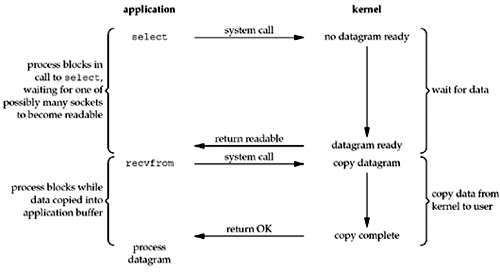
\includegraphics[width=.9\textwidth]{figs/06fig03.png}
  \end{center}
\end{frame}

\begin{frame}
\frametitle{Signal driven I/O Model}
  \begin{center}
  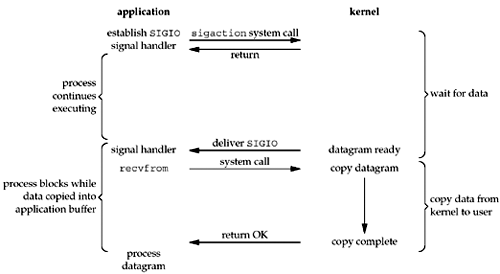
\includegraphics[width=.9\textwidth]{figs/06fig04.png}
  \end{center}
\end{frame}

\begin{frame}
\frametitle{Asynchronous I/O Model}
  \begin{center}
  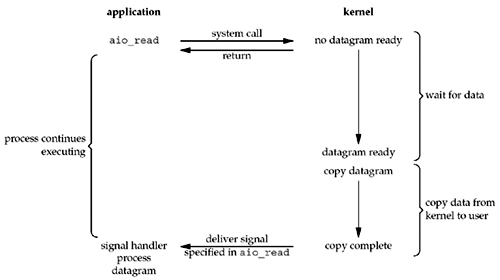
\includegraphics[width=.9\textwidth]{figs/06fig05.png}
  \end{center}
\end{frame}

\begin{frame}
\frametitle{Comparison of I/O Models}
  \begin{center}
  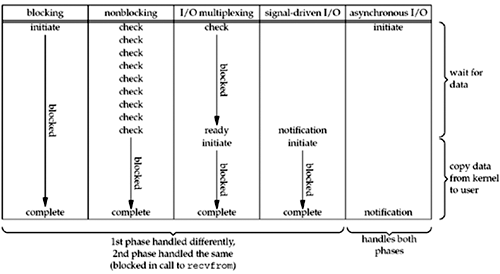
\includegraphics[width=.9\textwidth]{figs/06fig06.png}
  \end{center}
\end{frame}

\subsection{\texttt{select} Function}
\begin{frame}[containsverbatim]
\frametitle{\texttt{select} Function}
\begin{itemize}
  \item Allows the process to instruct the kernel to wait for any one of multiple events
  to occur and to wake up the process only when one or more of these events
  occurs or when a specified amount of time has passed.
  \item (readable, writable, expired time)
\end{itemize}
{\scriptsize
  \begin{verbatim}
#include <sys/select.h>
#include <sys/time.h>

int select(int maxfdp1, fd_set *readset, fd_set *writeset,
               fd_set *exceptset,
               const struct timeval *timeout);
  \end{verbatim}
}
\end{frame}

\begin{frame}[containsverbatim]
\frametitle{Descriptor sets}
\begin{itemize}
  \item Array of integers: each bit in each integer correspond to a descriptor.
  \item \texttt{fd\_set}: an array of integers, with each bit in each integer corresponding to a
descriptor.
\end{itemize}
{\scriptsize
\begin{verbatim}
 /* clear all bits in fdset */
 Void FD_ZERO(fd_set *fdset);
 /* turn on the bit for fd in fdset */
 Void FD_SET(int fd, fd_set *fdset);
 /* turn off the bit for fd in fdset*/
 Void FD_CLR(int fd, fd_set *fdset);
 /* is the bit for fd on in fdset ? */
 int FD_ISSET(int fd, fd_set *fdset);
\end{verbatim}
}
\end{frame}

\begin{frame}
\frametitle{Conditions Summary}
  \begin{center}
  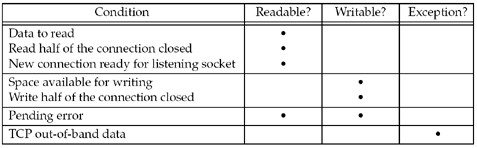
\includegraphics[width=.9\textwidth]{figs/06fig07.png}
  \end{center}
\end{frame}

\begin{frame}
\frametitle{\texttt{str\_cli} Function (Revisited)}
  \begin{center}
  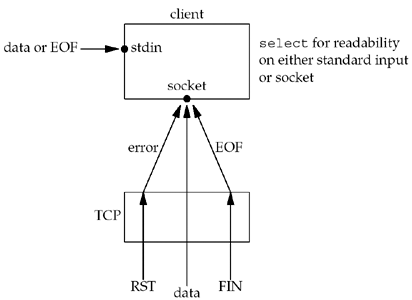
\includegraphics[width=.6\textwidth]{figs/06fig08.png}
  \end{center}
  Conditions handled by \texttt{select} in \texttt{str\_cli}.
\end{frame}

% \subsection{Batch Input and Buffering}
\begin{frame}
\frametitle{Batch Input and Buffering}
\begin{itemize}
  \item Network pipe is not fully used
\end{itemize}
 \begin{center}
  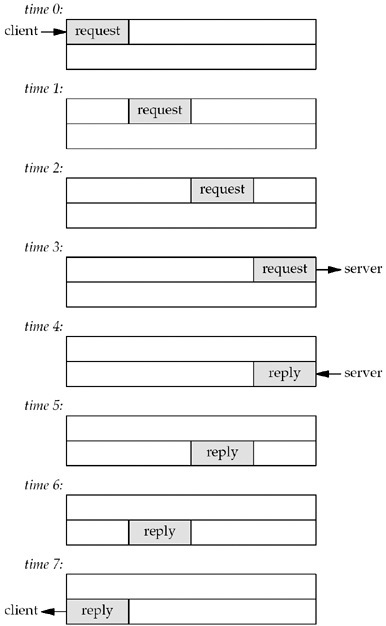
\includegraphics[width=.3\textwidth]{figs/06fig10.png}
  \hspace{2em}
  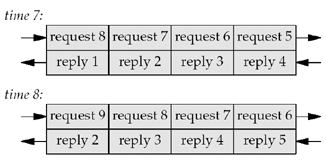
\includegraphics[width=.6\textwidth]{figs/06fig11.png}
  \end{center}
\end{frame}

% \subsection{\texttt{shutdown} Function}
\begin{frame}
\frametitle{\texttt{shutdown} Function}
 \begin{center}
  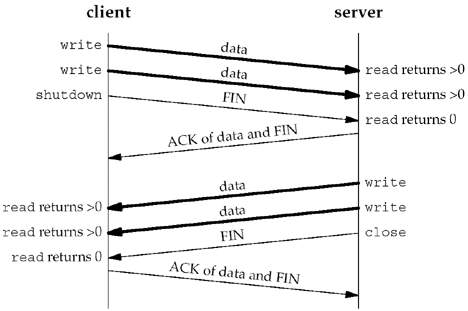
\includegraphics[width=.7\textwidth]{figs/06fig12.png}
  \end{center}
\end{frame}

\subsection{\texttt{pselect} Function}
\begin{frame}[containsverbatim]
\frametitle{\texttt{pselect} Function}
\begin{itemize}
  \item \texttt{pselect} function was invented by Posix.1g.
\end{itemize}
{\scriptsize
\begin{verbatim}
#include <sys/select.h>
#include <signal.h>
#include <time.h>

int pselect(int maxfdp1, fd_set *readset, fd_set *writeset,
                fd_set *exceptset, const struct timespec *timeout,
                const sigset_t *sigmask)

\end{verbatim}
}
\end{frame}

\subsection{\texttt{poll} Function}
\begin{frame}[containsverbatim]
\frametitle{\texttt{poll} Function}
\begin{itemize}
  \item Similar to select, but provide additional information when dealing with streams devices
\end{itemize}
{\scriptsize
\begin{verbatim}
#include <poll.h>
int poll(struct pollfd  *fdarray, unsigned long nfds, int timeout);
/*return : count of ready descriptors, 0 on timeout, -1 on error*/
\end{verbatim}
}
\end{frame}
%%
%\begin{frame}
%\frametitle{...}
%\begin{itemize}
%  \item
%  \item
%  \item
%  \item
%  \item
%\end{itemize}
%\end{frame}

\end{document}
